\documentclass[border=4pt]{standalone}
\usepackage{amsmath,amssymb,tikz}
\definecolor{figB}{RGB}{31,90,166}\definecolor{figR}{RGB}{176,48,48}\definecolor{figG}{RGB}{46,125,50}\definecolor{figO}{RGB}{214,120,20}
\begin{document}
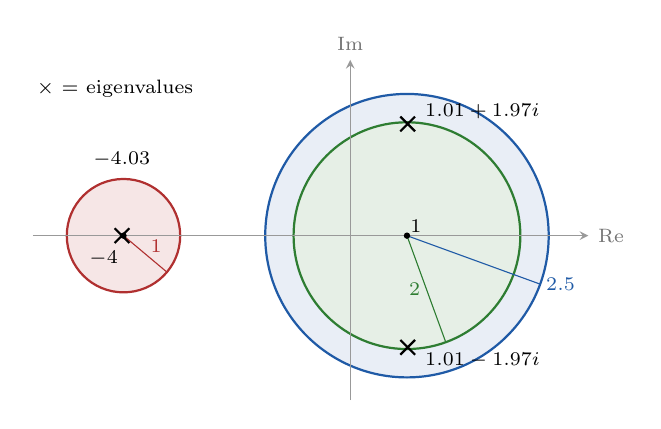
\begin{tikzpicture}[scale=0.72]
% disks: row 2 (radius 2.5), row 1 (radius 2), row 3 (radius 1)
\fill[figB!10] (1,0) circle (2.5); \draw[figB,thick] (1,0) circle (2.5);
\fill[figG!12] (1,0) circle (2);   \draw[figG,thick] (1,0) circle (2);
\fill[figR!12] (-4,0) circle (1);  \draw[figR,thick] (-4,0) circle (1);
\draw[thin,black!40,-stealth] (-5.6,0)--(4.2,0) node[right,font=\scriptsize,black!55]{$\operatorname{Re}$};
\draw[thin,black!40,-stealth] (0,-2.9)--(0,3.1) node[above,font=\scriptsize,black!55]{$\operatorname{Im}$};
% radii
\draw[figG,thin] (1,0)--++(-70:2) node[pos=0.5,left,font=\scriptsize,inner sep=2pt]{$2$};
\draw[figB,thin] (1,0)--++(-20:2.5) node[pos=1,right,font=\scriptsize,inner sep=2pt]{$2.5$};
\draw[figR,thin] (-4,0)--++(-40:1) node[pos=0.55,above right,font=\scriptsize,inner sep=1pt]{$1$};
% centres
\fill (1,0) circle (1.6pt) node[above right,font=\scriptsize,inner sep=1pt]{$1$};
\fill (-4,0) circle (1.6pt); \node[font=\scriptsize] at (-4.35,-0.4) {$-4$};
% eigenvalues
\foreach \p in {(1.013,1.970),(1.013,-1.970),(-4.026,0)} \draw[black,thick] \p ++(-0.13,-0.13)--++(0.26,0.26) \p ++(-0.13,0.13)--++(0.26,-0.26);
\node[font=\scriptsize,right] at (1.15,2.2) {$1.01+1.97i$};
\node[font=\scriptsize,right] at (1.15,-2.2) {$1.01-1.97i$};
\node[font=\scriptsize,above] at (-4.03,1.05) {$-4.03$};
\node[font=\scriptsize,anchor=west] at (-5.7,2.6) {$\times$ = eigenvalues};
\end{tikzpicture}
\end{document}
